
\documentclass[letterpaper]{report}
\usepackage{mysphinx}
\pagestyle{normal}
\usepackage{graphicx}
\graphicspath{ {images/} }



\newcommand{\X}{\mathbf{x}}
\newcommand{\Y}{\mathbf{y}}
\newcommand{\R}{\mathbf{R}}
\newcommand{\err}{err_{\hat{f}}}


%\usepackage{natbib,alifeconf}
\usepackage{natbib,amsmath}
\usepackage[top=1.5in, bottom=1.5in, left=1.25in, right=1.25in]{geometry}

% for the results table
\usepackage{booktabs}
\usepackage{multirow,bigstrut}
\usepackage{tabu}


\usepackage{palatino}
\usepackage{pxfonts}
\usepackage{caption}
\usepackage{subcaption}

\usepackage{framed}
\setlength{\fboxsep}{10pt}
\setlength{\fboxrule}{1.5pt}


%\usepackage[urw-garamond]{mathdesign}
%\usepackage[T1]{fontenc}



%\usepackage{amsmath}

%% Macros
\newcommand{\mb}{\mathbf}


\DeclareSymbolFont{bbold}{U}{bbold}{m}{n}
\DeclareSymbolFontAlphabet{\mathbbold}{bbold}

%%



\title{Sequential Model-Based Optimization\\ {\small \textit{-- of --}} \\Expensive Blackbox Functions}
\author{Drew Blount \\
\mbox{}\\
Mathematics Department, Reed College\\
\\
dblount@reed.edu}

\begin{document}
\maketitle

\chapter*{Abstract}

This thesis discusses a general method for the global optimization of expensive blackbox functions: sequential model-based optimization. `SMBO' works by iteratively fitting a prediction model to available data, and analyzing that model to inform further data-gathering, so as to generate another model with even greater predictive power. By recursively iterating this process, using successive prediction models to bootstrap ever-better models, good solutions are found to hard optimization problems.

This thesis starts in mathematical statistics, and ends in computer science and software design. I will first describe the SMBO process in general: its history, applications, and relevance to optimization today. I will then rigorously present a paradigmatic example of SMBO, the `EGO Algorithm' of Jones et al. A major goal of this thesis is to build a robust implementation of sequential model-based optimization capable of optimizing real-world processes. Thus I also include a detailed methods section presenting my Python package, \texttt{smbo}, a modular SMBO framework. The full documentation of \texttt{smbo} is also included as an appendix.
\chapter{Introduction}

Sequential model-based optimization is an accurately named process, because it attempts to optimize functions by developing a sequence of models. The broad idea is this: you want to understand some process's global behavior from a few sample points, and you have a limited ability to collect more data--think of additional samples as available, but expensive. This is often the case with processes that are difficult to observe or simulate.

Given a few sample points, you use the available data to develop a model of the process's behavior.  With this model alone, you could perform simple \emph{model}-based optimization, using it to predict the locations of global optima. In \emph{sequential} model-based optimization, however, we use predictive models in a more clever, bootstrapping way: to predict what further data, if collected, would allow us to improve our model---and thus our predictive ability---the most. In other words, each model is used to generate another, better model. Global optima, or at least very good solutions, are then found by recursively improving the predictive ability of a model.

To make this process more tangible, consider the case of gold-mining, which is a surprisingly deep analogy to the kind of data mining which is explored in this thesis. Imagine that you are a gold-miner, and you own a claim to Valley X. You want to understand where in the valley you could find the most gold, where best to start a mine. Your mining company has drilled five exploratory shafts throughout the valley. You make a map of the valley's gold distribution based on these five samples.

Were you, the gold miner, only interested in model-based optimization, you would use this rudimentary map to predict where the most gold in the valley is, and start your mine there. Say, however, that you have enough resources to drill five more exploratory shafts first. The clever miner then asks themself, ``where should I drill the next exploratory shaft, to best learn about where the gold is most concentrated in the valley?" By leveraging what they have learned from the first five data points, the miner finds the region they would like most to learn about. After drilling the sixth hole in this region, the miner can improve their model of the gold distribution yet again, and ask the same question: ``where should I drill next, to best advance my search for the gold optimum?'' The goal of this thesis is to automate this decision-making process.

\section{Black-Box Functions}
A central notion to this thesis is that of black-box functions and their optimization. Though the black-box function is an intuitive concept for many mathematicians and scientists, I have found in discussing this thesis with others that it is an unfamiliar idea to the layperson, so I will spend a moment making all readers fully comfortable with the notion.

Simply put, a black-box function is a mysterious process that turns inputs into outputs. Though its inner workings are unknown to the user, it does operate by some hidden logic. The task of this thesis is to optimize the behavior of this process without direct access tot he hidden logic inside the black box.

Imagine a literal black box, with some sort of terminal or opening for receiving inputs. If things are put in this box, it spits something out. This thought experiment is illustrated in Fig. \ref{fig:black_box}.

\begin{figure}[h]
	\centering
	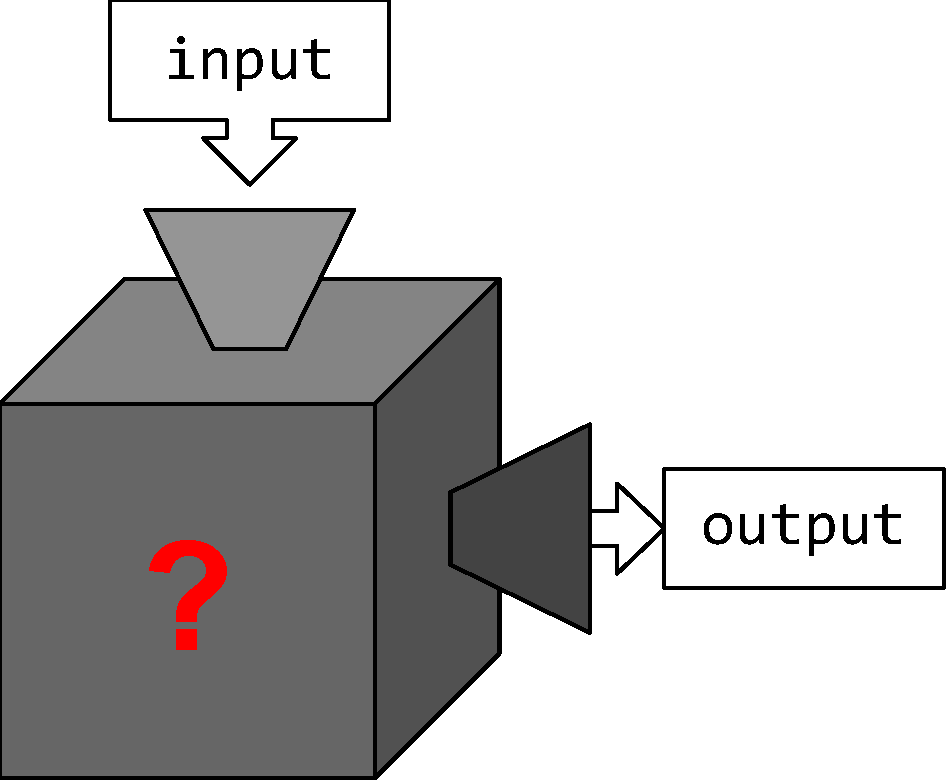
\includegraphics[width=0.5\textwidth]{images/blackbox}
	\caption{A black box: a mysterious but queryable function}
	\label{fig:black_box}

\end{figure}

Now imagine that you are confronted with a black box such as illustrated above, and in particular, one that produces a single numerical output when it is fed input\footnote{In this thesis, we are only concerned with functions that map some $k$ dimensions of input to a single-dimensional numeric output, as this is the standard model for optimization.}. Now imagine I were to assign you the task: in only twenty queries of the box, find a particular input that will induce an output greater than 100. How could you go about this task?

To make things easy, we'll make two assumptions about the hidden function in the box: that it is deterministic, so the same input will always produce the same output; and that similar inputs produce similar outputs. This second assumption is crucial, because it allows you to consider observed blackbox values to predict values you have not seen.

Given those two assumptions, no prior knowledge of the blackbox's workings, and the task, ``get the blackbox to produce a desirable output," what does one do? This thesis rigorously addresses that question.

Now this hypothetical, where you have found a magical box that has hidden math inside, and are for some cause compelled to wrench a desirable output from it, sounds somewhat cartoonish and abstract. Yet it is such a general framework, a huge range of real-world problems can be fit into its mould. How often do humans want to control a process that they do not understand, yet can experiment with? Consider the stock market: inputs are your trading decisions, the black box is the market, and the output is your profit. How many people would like a reliable optimization strategy for \emph{that} blackbox function? Many complex biochemical interactions are dynamical enough that they are extremely difficult to model and predict; one iconic example is of protein folding. Here, too, is a setting where inputs (chemical recipes) can be turned into outputs (chemical reagents, or perhaps biomedical results), though the mechanism that accomplishes that transformation (dynamic chemical reaction networks) is somewhat opaque in its inner workings. 

Another major application of blackbox optimizers, which will be explored further in the conclusion, is that of optimizing the parameters of yet other machine learning algorithms. This task, the problem of \emph{hyperparameter optimization}, seeks to optimize the blackbox function which maps algorithm configurations to algorithm performance. Given a machine learning problem, say, identifying dogs in photographs, it is usually fairly straightforward to a practitioner to decide on a class of algorithm that is well-suited to accomplishing that task, e.g., recurrent neural networks. Simply deciding on a class of solution algorithms is not enough to find a solution, however, as there are invariably a basketful of algorithm parameters which must be set before any learning is even to take place. For example, say you want to solve a problem with a so-called deep neural network: how do you decide how many layers of neurons to include? How many neurons should be in each layer? How do you choose an appropriate learning rate? An intuition for questions like these is a large part of what `expertise' means in the field of machine learning, but it is commonly acknowledged that such expertise often errs on artistry rather than science. Because machine learning systems are big, complex, dynamical (and perhaps emergent) systems, is is very hard to know beforehand how well a certain parameter set will solve a given problem or class of problems. Thus, the selection of hyperparameters is another problem space ripe for sequential model-based optimization.

\section{History}


[Just a few paragraphs here, talk first about actual kriging (which was done for gold) and maybe get a fun historical anecdote] \cite{cressie_kriging_1990}.

[Talk about the EGO paper \cite{jones_efficient_1998}--Hutter calls it the beginning of SMBO, ``limited to optimizing continuous parameters for noise-free functions (i.e., the performance of deterministic algorithms).'' \cite{hutter_sequential_2011} See citation for further discussion of SMBO history. Talk about the background of EGO authors, how Jones worked for GM and one of the case studies in the original paper involved 3D engine component design.]

Mention ``PDT$^{TM}$,'' ProtoLife's ``predictive design technology,'' which is illustrated by a figure very similar to Fig \ref{fig:smbo_cycle} \cite{protolife_pdt_2013}

Talk about Hutter's recent work, maybe Google talk? Perhaps some words about how the ML community isn't particularly interested right now, and is more interested in accomplishing extremely huge-dimensional mapping problems like vision and translation, which are being accomplished by deep nets.





\chapter{The SMBO Paradigm}\label{ch:smbo}

To formalize the notion of blackbox optimization, consider an expensive blackbox function $f$. I will also refer to $f$ as the \emph{objective function}, a term from the optimization and statistics communities. Say that $f$ has been evaluated on the inputs, or \emph{sample points}, $x_1,\ x_2, ... ,\ x_n$. These evaluations produce the observed outputs $y_i=f(x_i)$. If $\mb{x}=\{x_1, ... ,\ x_n\}$ and $\mb{y}=\{y_1, ...,\ y_n\}$, I'll refer to the pair $(\mb{x},\mb{y})$ as the \emph{sample data}. Because we are concerned with global optimization---without loss of generality, say minimization\footnote{In the optimization community, it is common to speak only of minimization, and the two words are used somewhat interchangeably. For example, the most popular Python library for optimization, \texttt{scipy.optimize}, contains only minimization routines. Of course, the task of maximizing a function $f$ is the same as minimizing its negative $-f$. }---the goal is to find an $x$ such that $f(x)<f(x')\ \ \forall\ x' \ne x$, while evaluating $f$ as few times as possible. This chapter describes formally how the SMBO process addresses this challenge. I will define notation as it is introduced, though for reference I have included a reference table of variable names and definitions in Figure \ref{fig:notation} below.
% Where does this important aside go?: It should be clear that, unless you have evaluated the black box function $f$ at every possible $x$, it is impossible to say with absolute certainty whether a given point is the global minimum. Thus, the goal of a statistical global optimization routine is to produce a candidate optimum $x$, with some measure of confidence that $x$ is in fact the global optimum.

\begin{minipage}{\textwidth}
\begin{framed}
\begin{description}
  \item[$f$]: the objective function
  \item[$k$]: the dimensionality of $f$'s domain space
  \item[$n$]: the number of sample points (points at which $f$ has been evaluated and $f(x)$ is known)
  \item[$x_i$]: the $i$th sample point (a $k$-vector)
  \item[$y_i$]$:= f(x_i)$; the known objective output at the $i$th sample point
  \item[$\X$]: the vector of sample points ($n$ $k$-vectors, an $n\times k$ matrix)
  \item[$\Y$]: the vector of known outputs (an $n$-vector).
  \item[$\hat{f}$]: the $k$-to-$1$-dimensional predictor function
  \item[$\err$]: the predicted error of $\hat{f}$; also a $k$-to-$1$-dimensional function
  \item[$y(x)$]$:=$Normal$(\hat{f}(x),\err(x))$; the random variable representing the predicted function distribution at x
\end{description}

\end{framed}
\captionof{figure}{Notation used throughout this thesis}
\label{fig:notation}
\end{minipage}

\section{The SMBO Loop}

`SMBO' describes an entire class of algorithms, rather than one in particular \cite{hutter_sequential_2011, hamadi_autonomous_2012, jones_efficient_1998, rasmussen_gaussian_2006}. %note: get more specific with those cites. should be a handful of specific papers presenting particular SMBO things
These algorithms differ along several dimensions: in their assumptions regarding determinism, the types of objective functions they can optimize, their modelling strategies, and the details of their interactive relationship to the objective functions being optimized, to name several. % clarification: such as some algorithms selecting one sample point, others more.
Across these differences, the defining feature of sequential model-based optimization can be described as a three-part loop, shown below.

\begin{minipage}{\textwidth}
\begin{framed}

\begin{enumerate} 
\item The objective function $f$ is evaluated at a set of input values $\mb{x}$, producing observed outputs $\mb{y}$.
\item A prediction model of the objective function, the ``predictor function'' $\hat{f}$ is fit to the sample points $(\mb{x},\mb{y})$, as well as a model of the expected error of $\hat{f}$, $\err$.
\item From considering the prediction surface and its error, $(\hat{f},\err)$, new input points $\mb{x_{new}}$ are chosen to be evaluated by $f$. These points are chosen to most improve the ability of the model $\hat{f}$ to find the global optimum.\end{enumerate}
\end{framed}

\captionof{figure}{The three-stage SMBO loop}
\label{fig:smbo_loop}
\end{minipage}
I'll call this three-part process the \emph{SMBO loop} or \emph{cycle}; it will be referenced throughout this thesis. 

Note that at every iteration of the SMBO loop, (presuming we are minimizing $f$) there is a current `incumbent minimum', the best sample point evaluated so far. I will denote this point $x_{min}$, and its associated objective value $y_{min}$:

\begin{align} \label{x_min}
x_{min} &= x_j \in \mb{x}\ |\ y_j \leq y_i\ \ \forall\ y_i \in \mb{y}\\
y_{min} &= f(x_{min}).
\end{align}

The SMBO loop returns $(x_{min},y_{min})$ once $y_{min}$ is satisfactory, which could be defined one of two obvious ways. If we are looking only for `good enough' performance in the blackbox function, then the halting criteria is once the incumbent $y_{min}$ drops below a set threshold, e.g., ``run the SMBO loop until you can find a blackbox value lower than $2$.'' Note that in general with a blackbox function, you can never be certain to have found the global optimum, unless you have sampled every point in the function's domain. Thus, the alternative to using a $y_{min}$ threshold as a halting criteria must be probabilistic---as will be described further in Section \ref{sec:max_imp}, from the prediction surface and its error function $(\hat{f},\err)$, we can rigorously predict the probability that the current $y_{min}$ is in fact the function's global minimum. Thus, it is straightforward to say, ``run the SMBO loop until you are 95\% confident that you have found the global minimum.''

\section{Visualizing the SMBO Loop}

The cyclical nature of sequential model-based optimization suggests a popular illustration of the method, which highlights how the three steps reinforce each other to generate successively more predictive models---see Figure \ref{fig:smbo_cycle}, below. It is somewhat notable that illustrations quite similar to Fig. \ref{fig:smbo_cycle} appear throughout the literature related to SMBO \cite{hutter_sequential_2011,protolife_pdt_2013}. This image is perhaps the most popular conceptualization of the SMBO method.

\begin{figure}[h]
	\centering
	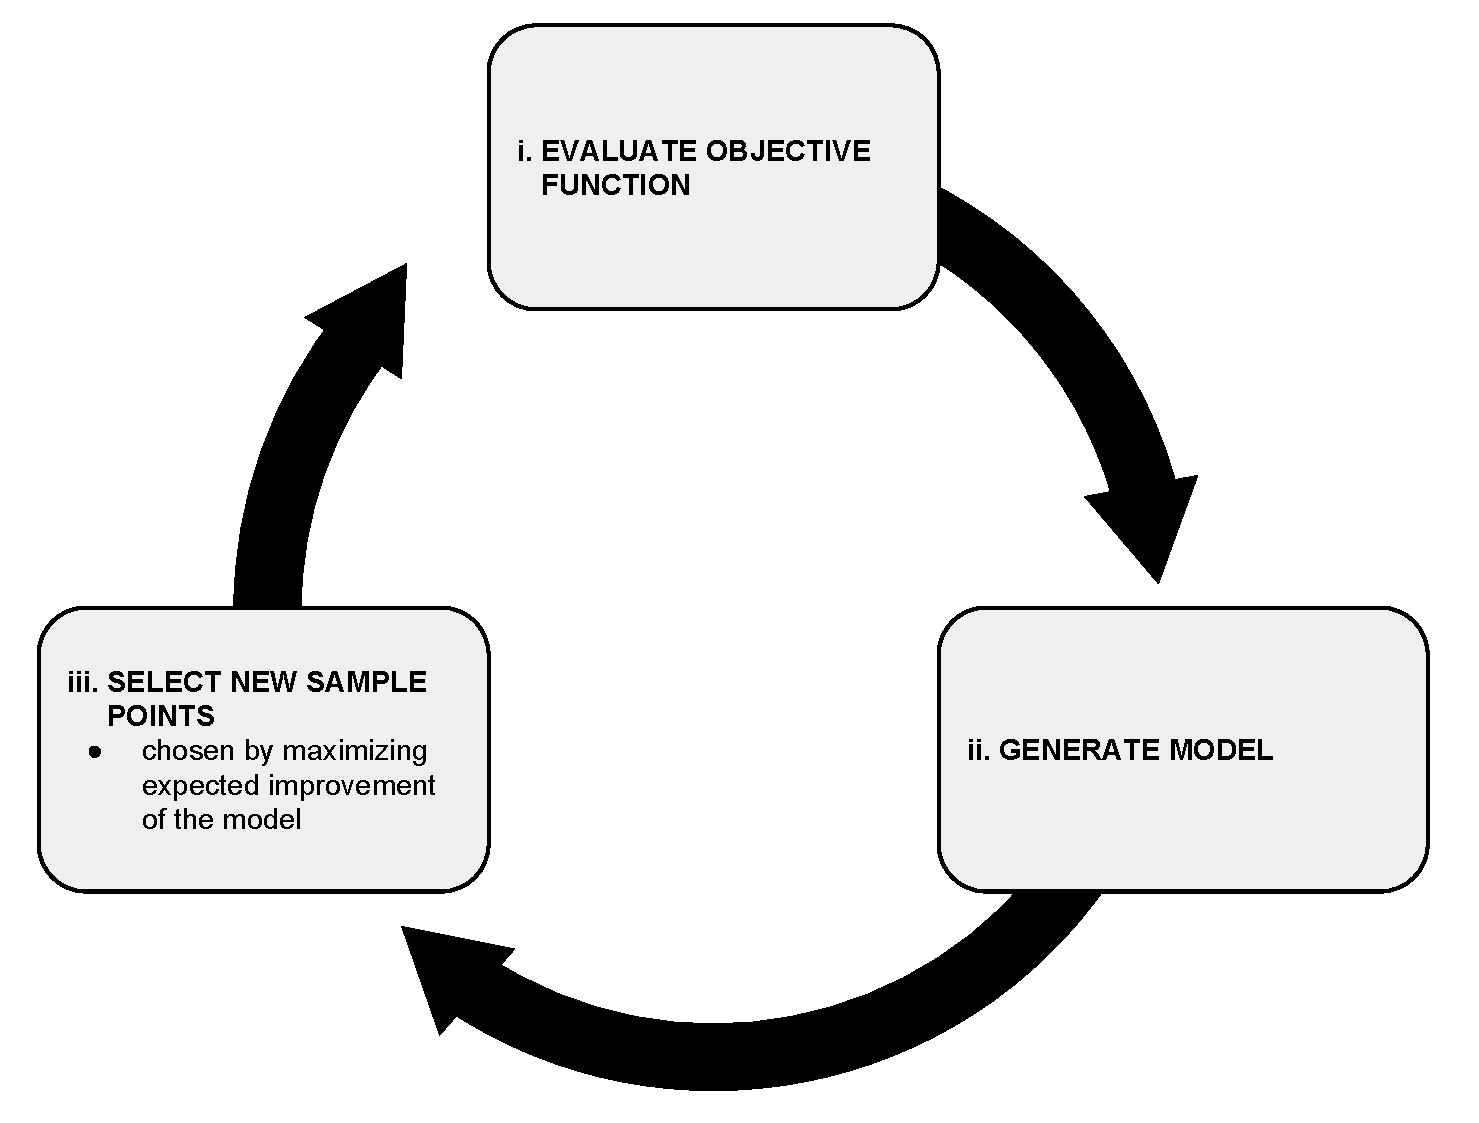
\includegraphics[width=0.75\textwidth]{images/smbo_loop}
	\caption{A popular visualization of the SMBO process. The methodology of node iii is largely fixed across different SMBO algorithms, while the details of Node ii are generally the distinguishing factors between different SMBO algorithms.}
	\label{fig:smbo_cycle}

\end{figure}


%In the vocabulary of above, each stage in the SMBO loop can be defined as a mathematical function:
%\begin{description}
%	\item[\textbf{I}]: The objective function maps $k$-vectors from input-space to outputs.
%	\item[\textbf{II}]: The model module maps the sample points to a model function.
%	\item[\textbf{III}]: The sampling strategy is a function that takes as input a model function, and outputs the next $k$-vector(s) which should be evaluated by the objective.
%\end{description}

%Seeing each component as simply a function mapping a certain kind of input to a certain kind of output, combined with the circular relationship illustrated in Fig \ref{fig:smbo_cycle}, is what motivates me to describe the SMBO process as bootstrapping. From the perspective of node \textbf{I} in the cycle, the output of the objective function determines the next input of the objective function, which determines the next input, and do on. From the perspective of node \textbf{II}, each model induces the model that follows it.

\section{SMBO$_{\text{III}}$: Maximum Improvement}\label{sec:max_imp}

The third step in the SMBO loop is perhaps the most characteristic---different SMBO algorithms use different model functions to accomplish the task in node \textbf{II}, and of course each implementation might attempt to optimize a unique objective function in step \textbf{I}. The third step, however, has a standard solution that is relatively ubiquitous: maximizing a function of input space called \emph{expected improvement}. 

There is a classical problem in optimization, of balancing the competing desires for exploration and exploitation \cite{John Holland}. Here, exploration refers to the impulse to sample in unknown regions of the objective function's domain, to learn more about its global behavior. Exploitation means the impulse to take advantage of what we already know, and sample where we predict we will find the global optimum. Expected improvement is one of those results from statistics that does a strikingly good job of quantifying a concept that seems at first to be too subtle to be easily quantified---it provides a satisfying solution to the exploration/exploitation conundrum.

Remember that during the SMBO process (as in many other optimization strategies), there is at all times a current ``incumbent optimum,'' $(x_{min},y_{min})$, which is the most optimal sample point evaluated so far. Simply put, the expected improvement of $x'$ measures amount by which we predict that $f(x')$ would be more optimal than $y_{min}$. More rigorously, improvement $I$ is defined as,

\begin{equation} \label{eq:improvement}
I(x) = min(y_{min}-y(x),0),
\end{equation}
where I have defined $y(x)=\text{Normal}(\hat{f}(x),\err(x))$; thus $I$ is a random variable. It should be clear to the reader that $I$ does capture the intuitive notion of improvement---it is the amount by which $y(x)$ is better than the incumbent optimum.

From this definition of improvement, all that is left is to apply the basic statistical notion of the expected value of a random variable to Eq. \ref{eq:improvement} to find the expected improvement function $\mb{E}[I(x)]$. Doing this, along with what \cite{jones_efficient_1998} calls `some tedious integration by parts,' produces the formula,

\begin{equation} \label{eq:exp_improvement}
\mb{E}[min(y_{min}-y(x),0)]=(y_{min}-\hat{f}(x))\times\Psi\left(\frac{y_{min}-\hat{f}(x)}{\err(x)}\right) + \err(x)\times\psi\left(\frac{y_{min}-\hat{f}(x)}{\err(x)}\right),
\end{equation}
where $\Psi$ and $\psi$ denote the standard normal distribution and density functions, familiar from statistics.

A significant feature of expected improvement is that it is monotonic in both $\err$ and $\hat{f}$. Ignoring $\hat{f}(x)$, if a prediction is uncertain (measured by $\err(x)$), then the expected improvement will be large. On the other hand, if we ignore predicted error, it is obvious that the points in input space where $\hat(x)$ is lower will have a higher expected improvement (assuming the goal is minimization). 

By choosing sample points to maximize the expected improve function, exploration and exploitation go hand in hand. This is easier illustrated than described, so I have included in Figure \ref{fig:explore_exploit} the plots from a toy SMBO instance where the exploration/exploitation distinction is was especially prominent.


\begin{figure}
\centering
\begin{tabular}{lr}
\subcaptionbox{The initial model, fit only on a 4-point latin hypercube sample.}
{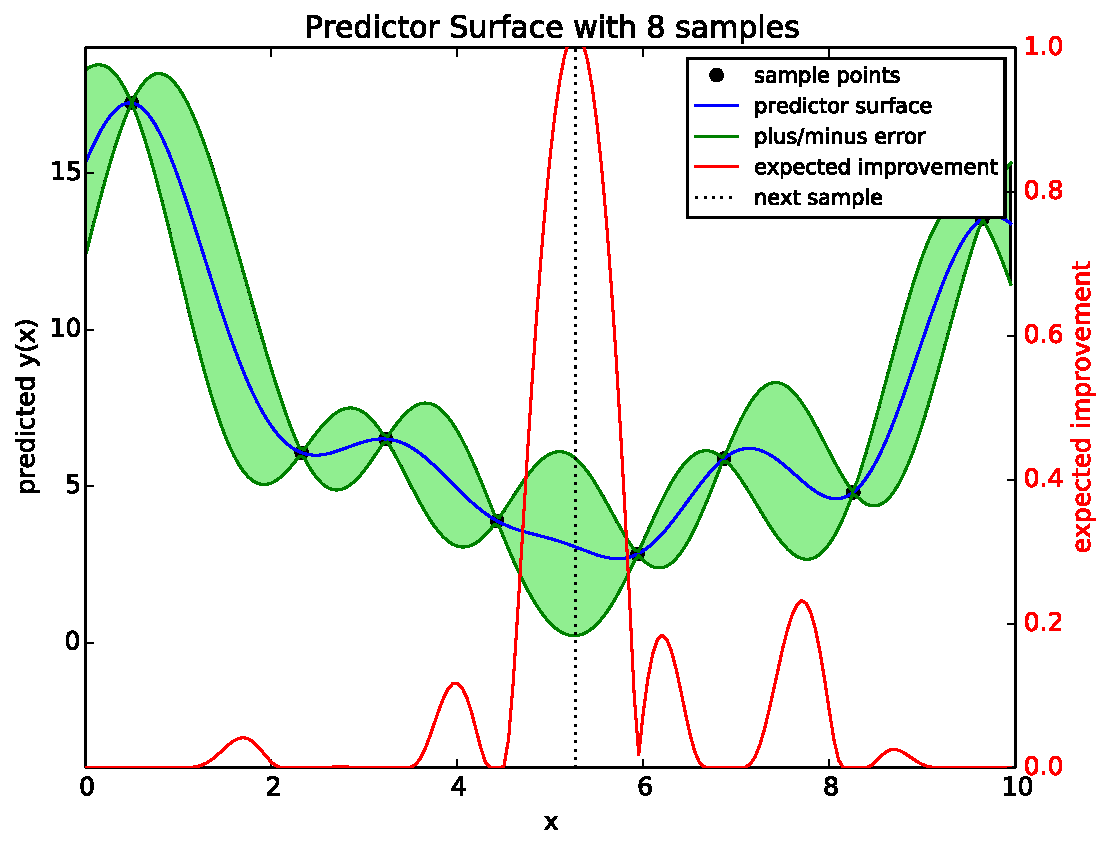
\includegraphics[width=0.4\textwidth]{images/ego_ex/0}} &

\subcaptionbox{Note that the new sample point is very near the global minimum.}
{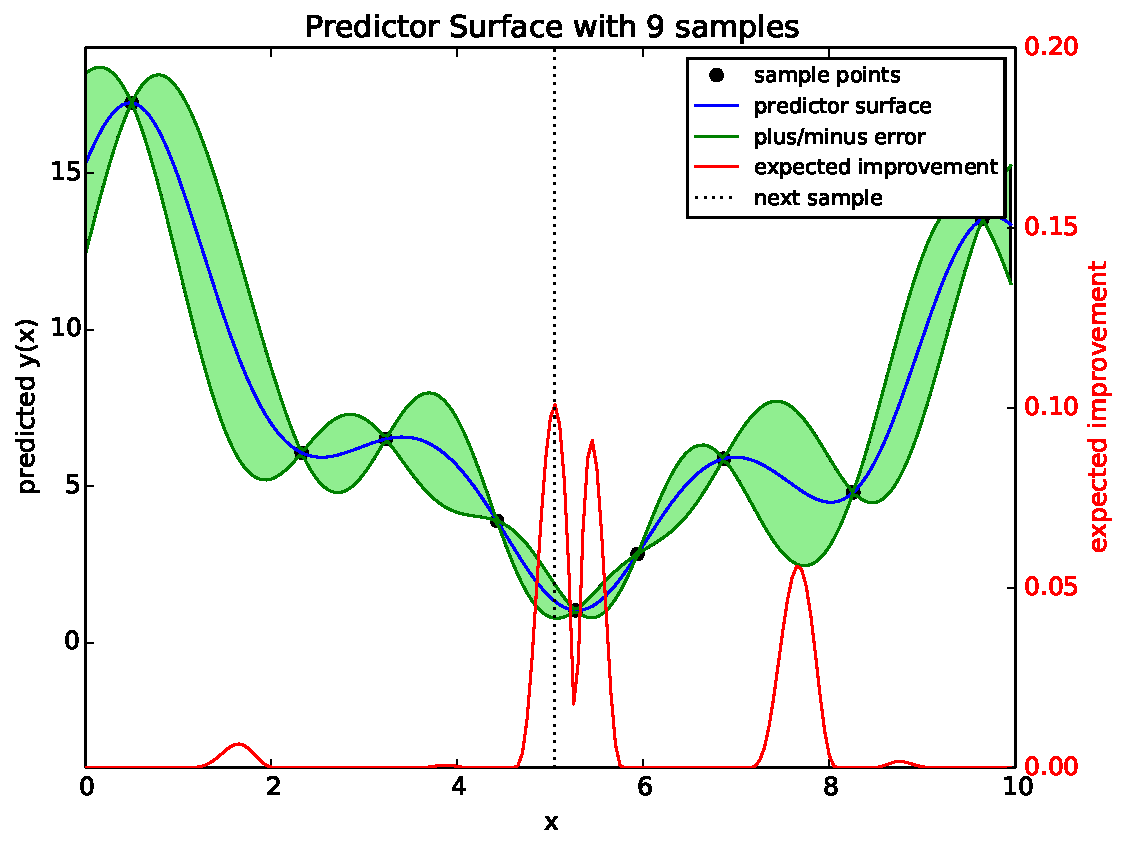
\includegraphics[width=0.4\textwidth]{images/ego_ex/1}}\\

\subcaptionbox{Despite the good result found in (b), the predictor is very uncertain in the unexplored region, so the expected improvement is largest there---it is now exploring rather than exploiting.}
{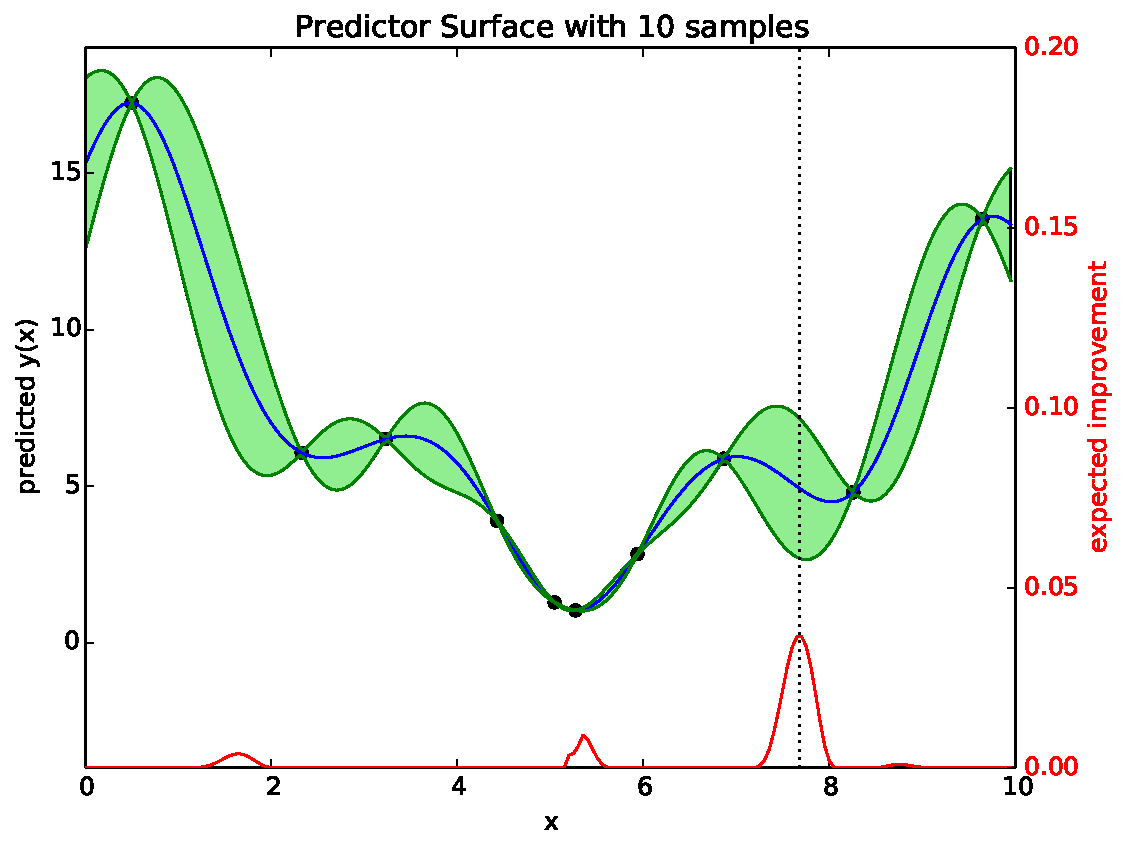
\includegraphics[width=0.4\textwidth]{images/ego_ex/2}} &

\subcaptionbox{More exploration of the uncertain region}
{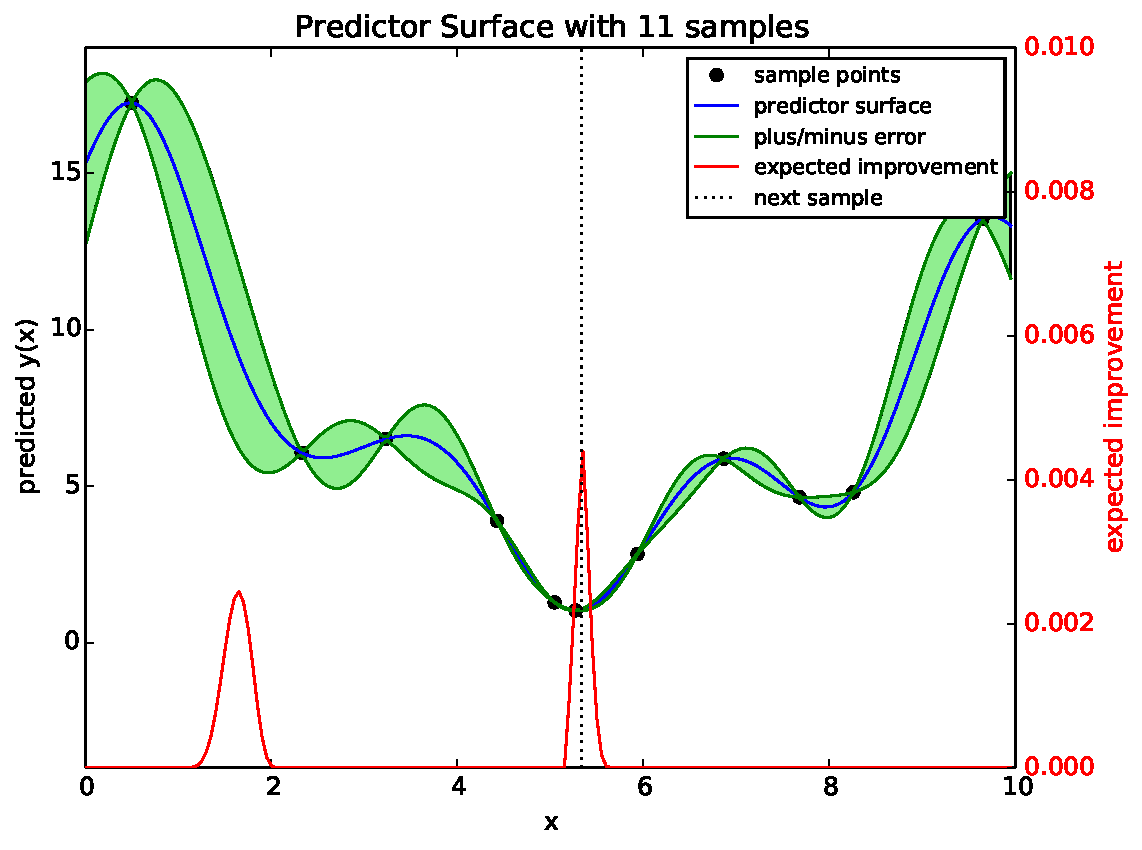
\includegraphics[width=0.4\textwidth]{images/ego_ex/3}}\\

\subcaptionbox{Now that the domain is more fully mapped, the algorithm is more confident that the solution in (b) is close to the global minimum}
{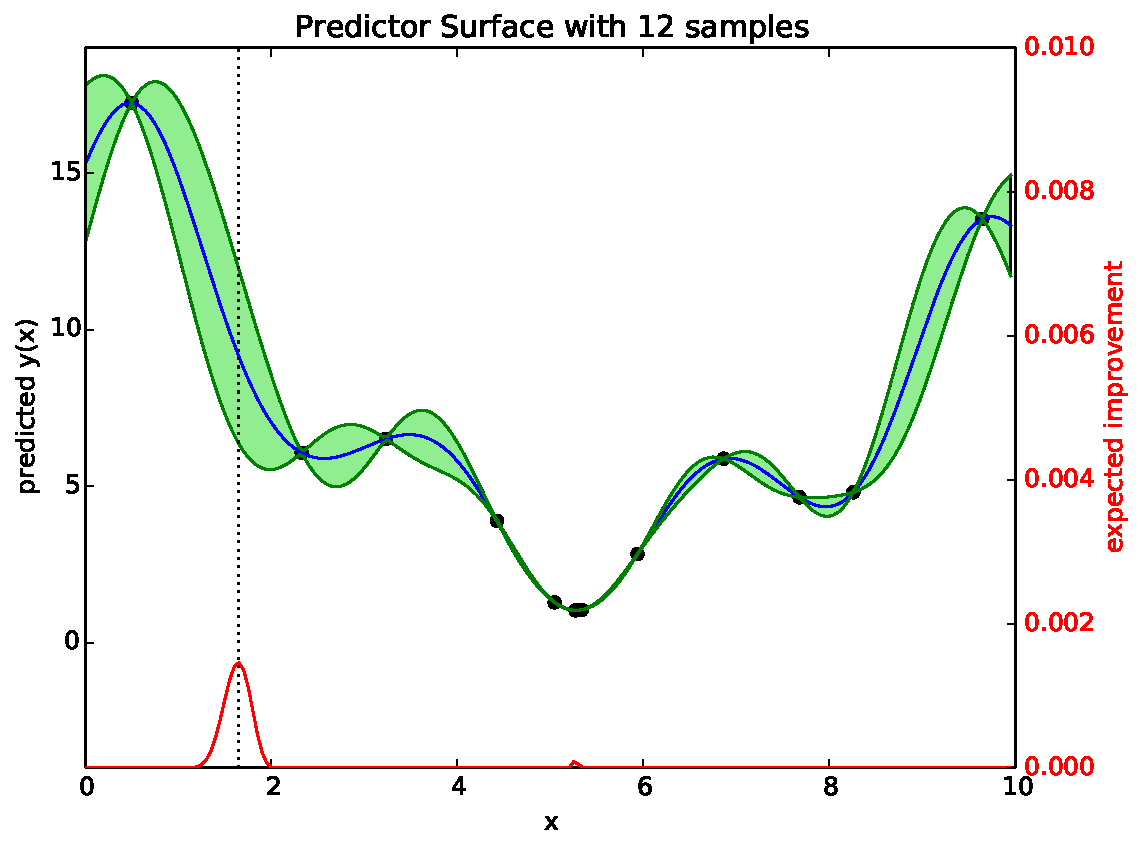
\includegraphics[width=0.4\textwidth]{images/ego_ex/4}} &

\subcaptionbox{Note that despite uncertain regions of the prediction surface, nowhere is it very likely that a new sample would find a better $y_{min}$.}
{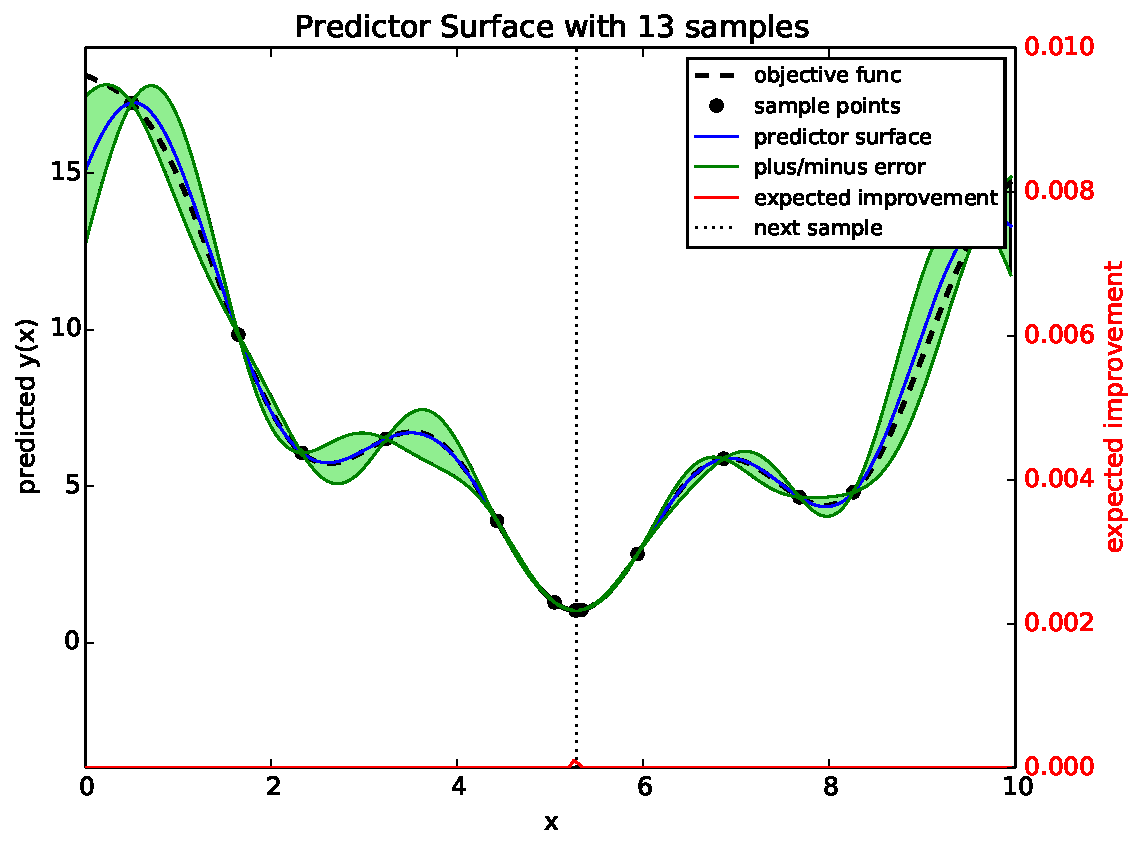
\includegraphics[width=0.4\textwidth]{images/ego_ex/5}}\\
\end{tabular}
\caption{An entire run of sequential model-based optimization of a toy function using the EGO algorithm, highlighting the exploration/exploitation tradeoff achieved by when maximum expected improvement is used to select $x_{new}$.}
\label{fig:explore_exploit}
\end{figure}


\section{SMBO$_0$: The Initial Sample}

Obviously, it is impossible to construct a model of a blackbox function's response surface if you have not ever queried the function at all, so the SMBO loop cannot start itself without a strategy for picking initial sample points. A popular strategy (find sources on wikipedia) for selecting these points, and the only strategy I will consider in this thesis, is called a latin hypercube sample. I will briefly describe it here, though the specific sampling method is not of great conceptual importance.

To construct an $n$-point latin hypercube in $k$ dimensions, first divide each dimension's domain into $n$ rows. This induces a grid, subdividing the original $k$-rectangular domain into $n^k$ sub-rectangles. A latin hypercube sample takes points from this domain under the constraint that no row in any one dimension contains two sample points.

That being said, the latin hypercube is one of those things that is more easily explained with pictures than words. [Put pictures here: is it cool to just life (and cite) the wikimedia commons pics from wikipedia?].

If you are a fan of sudoku, you have spent a lot of time thinking about latin hypercubes: the distribution of any one numeral across the game board matches a nine-sample two-dimensional latin hypercube. [Little picture demonstrating this, perhaps in a row with the wikipedia latin squares]








\chapter{Case study: the EGO Algorithm}\label{ch:ego}

The EGO algorithm is named for the paper in which it was presented, the informatively titled, ``Efficient Global Optimization of Expensive Blackbox Functions'' \citep{jones_efficient_1998}. I treat the EGO algorithm as the quintessential SMBO--it was the first, and it makes simple and intuitive assumptions about both the objective function and the best method to model it. [Kinda a lame explanation, but there has got to be more justification for treating EGO so centrally. One compelling thread is that the DACE model is provably the 'best linear unbiased predictor' (good wiki page on that)]. 

\section{The DACE Predictor}\label{sec:dace}
The model that is sequentially fit in the EGO algorithm is known as the DACE predictor. Like EGO, the DACE acronym comes from a somewhat generally-titled paper, in this case, ``Design and Analysis of Computer Experiments'' \citep{sacks_design_1989}. [Might want to elaborate later. For now, here's the bare info:] The assumptions that the DACE predictor makes are these (following closely Jones et al's presentation of DACE \cite{jones_efficient_1998}):

First, we assume what is called a \emph{stochastic process model} [get cites/explanation from Jones p.456], i.e., that,
\begin{equation} \label{eq:stoch_proc}
y(\X^{(i)}) = \mu + \epsilon(\X^{(i)}) \ \ \ \ \ \text{for } i \in (1,2,...,n).
\end{equation}
As is common in statistics, $\mu$ represents the mean of the process. Note that the above equation appears simpler than even linear regression, as it has no functional component. The DACE model, and stochastic processes in general, instead contains its predictive power in the `error terms' $\epsilon(\X^{(i)})$. These terms are assumed to be distributed normally,

\begin{equation} \label{eq:dace_err}
\epsilon(\X^{(i)}) = \text{Normal}(0,\sigma^2)\ \ \ \ \ \text{for } i \in (1,2,...,n),
\end{equation}

for a process-wide $\sigma^2$. Despite the normal distribution, the $\epsilon(\X^{(i)})$ are very much \emph{not} independent of each other: it is in a complex error-correlation structure that the DACE model encodes the contours of its response surface. Specifically,

\begin{equation} \label{eq:dace_corr}
\text{Corr}\left(\epsilon(\X^{(i)}),\epsilon(\X^{(i)})\right)\ \  = \ \ 
	\text{Exp}
		\left [ 
			-\sum_{h=1}^{k} 
				\theta_h \left | \X^{(i)}_h - \X^{(j)}_h \right | ^{p_h}
		\right ]\ \  = \ \ 
	\prod_{h=1}^{k}
		\text{Exp}
			\left [
				-\theta_h \left | \X^{(i)}_h - \X^{(j)}_h \right | ^{p_h}
			\right ],
\end{equation}

where the free parameters $\{(\theta_i,p_i)$ for $i \in (1,2,...,k)$ determine the shape of the DACE predictor. Note that these three constraints completely describe the DACE model: we assume that we are modeling a stochastic process with mean $\mu$, standard deviation $\sigma^2$, and inter-sample correlation described by Eq. \ref{eq:dace_corr}.

%write
Here I should discuss what error correlation means with some pretty pictures like in Jones p.459.

Much more can (and should, and will) be said about the shape of the predictor implied by this correlation equation, but for now it suffices to say that it encodes the heuristic, ``points near each other in input-space should have nearby function values'', with a concept of nearness along each input dimension that is gaussian in shape, with magnitude and falloff-steepness determined by $\theta$ and $p$.

\subsection{Selection of $\{(\theta_i,p_i)\}$}\label{sec:max_lik}
To fit a DACE predictor to sample data, the $k+2$ free parameters $\mu, \sigma^2,$ and $\{(\theta_i,p_i)\}$ for $i \in (1,2,...,k)$ are set by maximizing the likelihood function which is implied by the prior assumptions \ref{eq:stoch_proc, eq:dace_err, eq:dace_corr}. I will here walk through the derivation of that likelihood function.

Likelihood, I'll remind the reader, is a statistical concept very similar to probability. % get a dank intro stats textbook here.
Imagine a scenario where parameters $\psi$ give rise to some model $f_\psi$. Given some empirical observations $Z$, the concept of likelihood allows us to quantify how well the parameter choice $\psi$ and the generated model $f_\psi$ match our empirical observation---likelihood tests how well a model matches data. This is done quite simply: by defining the likelihood of a set of parameters given an observation, as the probability of that observation, given those parameters:

\begin{equation} \label{eq:def_likelihood}
L(\psi|Z) = Pr(Z|\psi).
\end{equation}

Note that this works intuitively well with our notion of probability: a set of parameters is a good one, i.e. it is likely, if the model that it generates is one wherein our observed data are relatively probable. The best model is that which is most likely, meaning that under no other model would the observed data $Z$ appear more probable.

Here, our observed data is the vector of witnessed function values $\Y$, so finding an equation for the likelihood of our parameters is equivalent to deriving the joint probability distribution of this $n$-vector, given the assumptions laid out in the previous section. I will now derive this joint distribution, using techniques that should be familiar to those schooled in college-level statistics. I'll first derive a simpler distribution, then use the change of variables formula to arrive at the result.

Consider a set of independent, identically-distributed gaussian random variables $\mathbb{Z} = Z_1,...,Z_n$, with mean 0 and standard deviation $\sigma^2$. For the sake of being explicit, the expectation function $f_{Z_i}$ for each $Z_i$ is then,

\begin{equation} \label{eq:f_{Z_i}}
f_{Z_i}=\frac{1}{\sigma\sqrt{2\pi}}e^{-Z_i^2/2\sigma^2}.
\end{equation}

The joint probability distribution of $\mathbb{Z}$ is simply the product of each of its [independent] components:

\begin{align}  \label{eq:F_Z}
f_\mathbb{Z}(\mathbb{Z}) &= \prod_{i=1}^n \frac{1}{\sigma\sqrt{2\pi}}e^{-Z_i^2/2\sigma^2}tf  \\
			 &= \frac{1}{(2\pi\sigma^2)^{n/2}} {E}xp\left [ -\frac{1}{2\sigma^2}\sum_{i=1}^{n} Z_i^2\right ] \nonumber\\
			 &= \frac{1}{(2\pi\sigma^2)^{n/2}} e^{-\mathbb{Z}^T\mathbb{Z}/2\sigma^2},\nonumber
\end{align}

where the last line uses vector multiplication to denote the sum of the square components of $\mathbb{Z}$.

Now, we use the change of variables formula to derive from this an equation for our actual data. For convenience, I'll consider the probability distribution of the vector of error terms, $\mathbb{\epsilon}$, rather than simply the output vector $\mathbbold{y}$. If $\mathbbold{1}$ denotes the 1-vector, then,

\begin{equation}\label{eq:epsilon}
\epsilon = \mathbbold{y} - \mathbbold{1}\mu.
\end{equation}

I will also consider $\mathbb{R}$, the \emph{correlation matrix} of the errors $\epsilon$. $\mathbb{R}$ is simply the $n\times n$ matrix whose $(i,j)^{th}$ entry is $Corr[\epsilon_i,\epsilon_j]$ as defined in Eq \ref{eq:dace_corr}. By construction, we know that $\mathbb{R}$ is symmetric and positive-definite, which means that a Cholesky decomposition exists CITE\cite{linear_algebra}, i.e., that there exists a lower-triangular matrix $A$ such that,

\begin{equation} \label{eq:cholesky}
\mathbb{R} = A A^T.
\end{equation}

Now, because of [WHY? is it the lower-triangularity of $A$? I don't see how we know that the difference between $\epsilon$ and iid is the matrix A], we know that,
\begin{equation} \label{Y_sub}
\epsilon=A\mathbb{Z},
\end{equation}

where $\mathbb{Z}$ is and independent, identically distributed vector with each component Normal$(0,\sigma^2)$. We will use this fact, along with the change of variables formula and the above-derived probability density function for such a $\mathbb{Z}$ (Eq \ref{eq:F_Z}), to arrive at the likelihood equation. Letting $g$ denote the linear transformation equivalent to left-multiplication by the matrix A, we see that,

\begin{align}
\epsilon &= g(\mathbb{Z}) \nonumber \\
\mathbb{Z} &= g^{-1}(\epsilon) = A^{-1}\epsilon
\label{eq:sub}
\end{align}



Now recall the change of variables formula, which given Eq. \ref{eq:sub} states that,
\begin{align} \label{eq:change_of_vars}
f_\epsilon &= f_\mathbb{Z}\left (g^{-1}(\mathbb{Z})\right)\times \left | g^{-1}(\mathbb{Z}) \right | \\
			 &= f_\mathbb{Z}\left (A^{-1}\epsilon\right) |A^{-1}| \\ 
			 &= f_\mathbb{Z}\left (A^{-1}\epsilon\right) \frac{1}{|A|}
\end{align}

Now plugging in Eq. \ref{eq:F_Z}, the formula for $f_\mathbb{Z}$, 

\begin{align} \label{eq:getting_F_Y}
f_\epsilon &= \frac{1}{(2\pi\sigma^2)^{n/2}|A|} {E}xp\left [ -\frac{1}{2\sigma^2}(A^{-1}\epsilon)^T(A^{-1}\epsilon)\right ].
\end{align}

Now I will do some linear algebra to the matrices in the exponent,

\begin{align}
(A^{-1}\epsilon)^T(A^{-1}\epsilon) &= \epsilon^T(A^{-1})^TA^{-1}\epsilon \nonumber\\
			 						 &= \epsilon^T((A^T)^{-1}A^{-1})\epsilon\nonumber\\
									 &= \epsilon^T(AA^T)^{-1}\epsilon\nonumber\\
									 &= \epsilon^T\mathbb{R}^{-1}\epsilon
									 \label{eq:inverse}
\end{align}

Using this result, and also rewriting $|A|$ as $|\mathbb{R}|^{1/2}$ (by Eq. \ref{eq:cholesky} and the fact that the determinant of a product is the product of the determinants), we get the clean formulation,

\begin{equation} \label{eq:likelihood1}
\frac{1}
  {(2\pi\sigma^2)^{n/2}|\mb{R}|^{1/2}}\ 
Exp \left 
  [ -\frac
    {\epsilon^T\mathbb{R}^{-1}\epsilon}
    {2\sigma^2} 
\right ],
\end{equation}

which was written by Jones et al as,

\begin{equation} \label{eq:likelihood}
\frac{1}
  {(2\pi\sigma^2)^{n/2}|\mb{R}|^{1/2}}\ 
Exp \left 
  [ -\frac
    {(\mb{y}-\mb{1}\mu)^T\mb{R}^{-1}(\mb{y}-\mb{1}\mu)}
    {2\sigma^2} 
\right ].
\end{equation}

If we fix the $\{(\theta_i,p_i)\}$, the above equation can be analytically maximized in $\mu$ and $\sigma^2$ \citep{jones_efficient_1998} to get,

\begin{equation} \label{eq:mu_hat}
\hat{\mu}=\frac
	{\mb{1}^T\mb{R}^{-1}\mb{y}}
	{\mb{1}^T\mb{R}^{-1}\mb{1}},
\end{equation}


and,

\begin{equation} \label{eq:sig_hat}
\hat{\sigma}^2
    = \frac{(\mb{y}-\mb{1}\hat{\mu})^T\mb{R}^{-1}(\mb{y}-\mb{1}\hat{\mu})}{n} 
	= \frac{\epsilon^T\mb{R}^{-1}\epsilon}{n}.
\end{equation}

Note that when $\mb{R}=\mb{I}$, the identity matrix, there is no correlation between each variable. As you would hope, in this case Eq. \ref{eq:mu_hat} and Eq. \ref{eq:sig_hat} reduce to the standard statistical definitions of mean and standard deviation.

By substituting Eq. \ref{eq:mu_hat} and Eq. \ref{eq:sig_hat} into the likelihood equation (Eq \ref{eq:likelihood}), we get the concentrated likelihood equation, which in practice is numerically maximized to fit the DACE parameters $p,\ \theta$:

\begin{equation} \label{eq:conc_likelihood}
\frac{e^{n/2}}
  {(2\pi\hat{\sigma}^2)^{n/2}|\mb{R}|^{1/2}},
\end{equation}

\chapter{A Python Package for SMBO} \label{ch:code}


In exploring this topic, I have built a Python package for performing sequential model-based optimization, simply named \texttt{smbo}. My goal in making it was to construct well-made code that will be immediately useful as a pedagogical tool (indeed, it was used to generate several figures in this thesis, such as those in Section \ref{sec:smbo_ex}), open source and available online, and documented and designed such that further development of the code base is easy. Perhaps some day \texttt{smbo} will evolve into a cutting-edge free optimization package, used to optimize all sorts of blackbox functions all over the globe, maintained by an international team of elite open-source hackers. Presently, the project is more humble. As of submitting this thesis, the package only implements the EGO algorithm, though its modular, hybrid object-oriented/functional construction allows for further SMBO processes to be defined and implemented easily. \texttt{smbo} is available on the Python Package Index, and can be downloaded and installed with a single command on any computer with Python 2.7.9 or later.\footnote{\texttt{sudo pip install smbo}}

As a good portion of the work in this thesis went into software design and engineering (subjects not taught at Reed College), I will here present the code behind the \texttt{smbo} package on the highest level. This discussion will inform the reader's mathematical understanding of SMBO processes, covering design decisions, identifying runtime bottlenecks, and the crucial components upon which the performance of any SMBO implementation rely. This chapter will also serve as an introduction to the official documentation of the \texttt{smbo} package, which is included as an appendix to this thesis.

\section{Design}\label{sec:design}

The three-stage SMBO cycle, illustrated earlier in Figure \ref{fig:smbo_cycle}, presents a clear opportunity for a modular package design. As a reminder to the reader, the SMBO loop has three parts: an objective function (i), a modelling method (ii), and a method for additional sample point selection (iii). I will present \texttt{smbo} as it relates to these three steps.

\subsection{\texttt{smb$\_$optimizer}}

The technical goal of the \texttt{smbo} package is to provide a class, called \texttt{smb$\_$optimizer}, which generically handles and passes arguments between each component of the SMBO loop to facilitate iteration of the SMBO process. Since this thesis is largely concerned with the case where (iii) is defined by expected improvement maximization (Section \ref{sec:max_imp}), this stage of the process is implemented by a fixed class method of \texttt{smb$\_$optimizer}, called \texttt{sample}. The other two steps of the loop are implemented as functional properties of each \texttt{smb$\_$optimizer} instance, passed as initialization arguments. This information is illustrated on the familiar SMBO loop in Figure \ref{fig:smbo_loop_II}. Figure \ref{fig:smb_opt_doc} is a summary of the official documentation for the \texttt{smb$\_$optimizer} class, listing all of the high-level methods used in iterating the SMBO loop.

\begin{figure}[h]
	\centering
	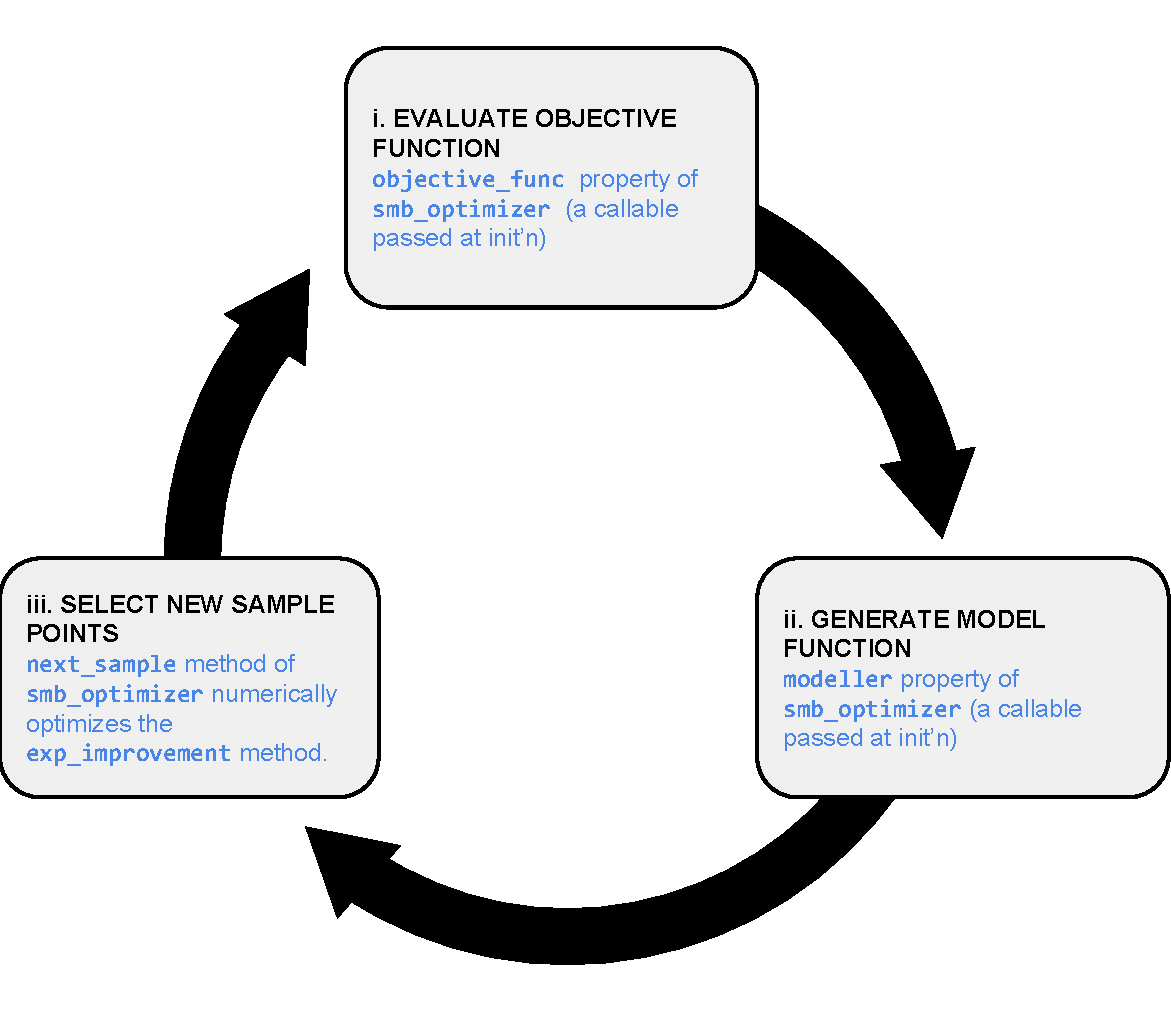
\includegraphics[width=0.75\textwidth]{smbo_loop_II}
	\caption{An instantiation of an SMBO process consists of a single \texttt{smb$\_$optimizer} object. Here the SMBO loop is labeled with the type of its implementation in the \texttt{smb$\_$optimizer} class.}
	\label{fig:smbo_loop_II}

\end{figure}


% The smb_optimizer documentation
\begin{minipage}{\textwidth}
\begin{framed}
\begin{fulllineitems}
\phantomsection\label{index:smbo.smb_optimizer.smb_optimizer}\pysiglinewithargsret{\strong{class }\code{smbo.smb\_optimizer.}\bfcode{smb\_optimizer}}{\emph{domain}, \emph{objective\_func}, \emph{modeller}, \emph{init\_sampler=None}}{}
An object that, given an input domain, objective function, and modelling strategy, implements sequential model-based optimization to search for a global minimum of the objective function.
\begin{quote}\begin{description}
\item[{Initialization Arguments}] \leavevmode\begin{itemize}
\item {} 
\textbf{\texttt{domain}} (\emph{list}) -- a list whose \(i^{th}\) element is the \((lower\ bound,\ upper\ bound)\) pair
describing the domain of interest in the \(i^{th}\) input dimension. The length
of this list defines the dimension of input space, denoted \(k\). This smb\_optimizer
then optimizes the \(k\)-rectangle defined by the domain arg.

\item {} 
\textbf{\texttt{objective\_func}} (\emph{function}) -- a function (or any object with a suitable \_\_apply\_\_ method)
that maps \(k\)-vectors to floats. The goal of an smb\_optimizer is to minimize this
function over the domain defined above.

\item {} 
\textbf{\texttt{modeller}} (\emph{function}) -- a function (or any object with a suitable \_\_apply\_\_ method) that maps a
tuple \((X,Y)\), which describes the input and known output values for a list of sample points to a tuple of functions
\((\hat{y},\ \hat{\sigma}^2)\).
\(\hat{y}\) represents the model's best estimate of \code{objective\_func(X)}, and \(\hat{\sigma}^2\)
is the estimated error of that prediction.

\item {} 
\textbf{\texttt{init\_sampler}} (\emph{function}) -- a function which will select initial sample points, informing the zero-generation model.
If left unspecified, is by default set to a \(2k+2\)-sample latin hypercube over the domain,
created with \code{smbo.latin\_hypercube}.

\end{itemize}


\item[{Attributes---Set at Initialization}] \leavevmode\begin{itemize}

\item{}
\textbf{\texttt{X}} (\emph{list}) -- The list of points where \code{objective\_func} has been evaluated already

\item {} 
\textbf{\texttt{Y}} (\emph{list}) -- The list of associated objective function values.

\item {} 
\textbf{\texttt{pred\_y}} (\emph{function}), \textbf{\texttt{pred\_err}} (\emph{function}) -- The predictor and predicted error surfaces; the output of \code{modeller(X,Y)}.

\item {} 
\textbf{\texttt{f\_min}} (\emph{dict:}\texttt{\{x:\_,y:\_\}}) -- The sample point that is the current known minimum.


\end{itemize}


\end{description}\end{quote}

% expected improvement
\index{exp\_improvement() (smbo.smb\_optimizer.smb\_optimizer method)}

\begin{fulllineitems}
\phantomsection\label{index:smbo.smb_optimizer.smb_optimizer.exp_improvement}\pysiglinewithargsret{\bfcode{exp\_improvement}}{\emph{x\_new}}{}Calculates the expected improvement at \code{x\_new}, by estimating from \code{pred\_y} and \code{pred\_err} the probability that an evaluation of \code{objective\_func} at \code{x\_new} would find a value lower than \code{f\_min}.


\end{fulllineitems}


% sample
\begin{fulllineitems}
\phantomsection\label{index:smbo.smb_optimizer.smb_optimizer.sample}\pysiglinewithargsret{\bfcode{sample}}{}{}
Chooses the next sample point by maximizing \code{exp\_improvement}.
Evaluates \code{objective\_func} there, updating \code{X} and \code{Y}. Updates \code{pred\_y} and \code{pred\_err} to the output of \code{modeller(X,Y)}.
\end{fulllineitems}


% take_samples
\index{take\_samples() (smbo.smb\_optimizer.smb\_optimizer method)}
\begin{fulllineitems}
\phantomsection\label{index:smbo.smb_optimizer.smb_optimizer.take_samples}\pysiglinewithargsret{\bfcode{take\_samples}}{\emph{stopping\_improvement=0.01}, \emph{max\_iters=100}, \emph{plot\_dims=None}}{}
Completes the SMBO loop until the best expected improvement is below \code{stopping\_improvement}, or \code{max\_iters} times. Optionally, produces plots of the prediction and error surfaces at every iteration.
\end{fulllineitems}






\end{fulllineitems}


\end{framed}

\captionof{figure}{A summary of the documentation of the \texttt{smb$\_$optimizer} class.}

\end{minipage}




The EGO algorithm, our prototypical SMBO process, is defined by a particular choice of modeller in ste (ii) of the loop, i.e., the DACE model. This is accomplished by a both a DACE function \emph{and} a class in the \texttt{smbo.modellers} module\footnote{The purpose of the \texttt{modellers} module of the \texttt{smbo} package is to contain various predictive models such as DACE, to serve as step (ii) in the SMBO loop.} This is the primary component of \texttt{smbo} meriting the description ``functional/object-oriented hybrid'' mentioned in the introduction to this chapter.

The class \texttt{dace$\_$model} has various methods to implement the calculations defined and derived in Chapter \ref{ch:ego}, including the formulation of $\hat{f}$ and $\err$. The \texttt{dace\_function} function maps the objective data $(\X,\Y)$ (stored here as properties of the $\texttt{smb\_optimizer}$ instance, \texttt{self.X} and \texttt{self.Y}\footnote{Note that in Python, \texttt{self} denotes the class instance at hand, like \texttt{this} in e.g. Java}) to the model functions $(\hat{f},\err)$, which are returned to the $\texttt{smb\_optimizer}$ and stored as \texttt{self.pred\_y} and \texttt{self.pred\_err}. This and more is illustrated in Figure \ref{fig:dace_doc}, a summary of the documentation for \texttt{dace\_function} and \texttt{dace\_model}. Note that the characteristic parameters $\{p_i\},\{\theta_i\}$ are stored as vectors by the \texttt{dace\_class}, in properties \texttt{self.P} and \texttt{self.Q}, respectively.



% The dace documentation
\begin{minipage}{\textwidth}
\begin{framed}
\begin{fulllineitems}
\phantomsection\label{index:smbo.models.dace}\pysiglinewithargsret{\strong{class }\code{smbo.models.}\bfcode{dace}}{\emph{X}, \emph{Y}}{}
A class that implements the DACE model to produce predictor and error surfaces from sample points
\begin{quote}\begin{description}
\item[{Parameters}] \leavevmode\begin{itemize}
\item {} 
\textbf{\texttt{X}} (\emph{list}) -- a list of input vectors

\item {} 
\textbf{\texttt{Y}} (\emph{list}) -- a list of observed objective values

\end{itemize}

\item[{Returns}] \leavevmode
(pred\_y,pred\_err): two functions, each k-to-1, where k is the dimension of the input space, representing the DACE predictor and predicted error at any point in input space.

\item[{Return type}] \leavevmode
tuple

\end{description}\end{quote}
\index{conc\_likelihood() (smbo.models.dace method)}

\begin{fulllineitems}
\phantomsection\label{index:smbo.models.dace.conc_likelihood}\pysiglinewithargsret{\bfcode{conc\_likelihood}}{\emph{new\_P=None}, \emph{new\_Q=None}}{}~\begin{quote}\begin{description}
\item[{Parameters}] \leavevmode\begin{itemize}
\item {} 
\textbf{\texttt{new\_P}} (\emph{list}) -- an \(n\)-vector resetting the \(p\) parameter of the DACE model

\item {} 
\textbf{\texttt{new\_Q}} (\emph{list}) -- an \(n\)-vector resetting the \(q\) or :math:{}`        heta{}` parameter of the DACE model

\end{itemize}

\end{description}\end{quote}

Returns the statistical likelihood of the current DACE parameters \code{P' and :code:{}`Q', given the data :code:{}`X} and \code{Y}.

\end{fulllineitems}
\end{fulllineitems}

\end{framed}

\captionof{figure}{A summary of the documentation of the \code{dace} model class. } \label{fig:dace_doc}

\end{minipage}

An \code{smb\_optimizer} class instance takes \code{dace\_function} (Fig \ref{fig:fig:dace_doc}) as its \code{modeller} argument. Even though the \code{smb\_optimizer} is only aware of this function, each function call initializes a \code{dace} object, which stays alive behind the scenes as long as its \code{predict} and/or \code{pred\_err} methods are being actively called, which is often, as these form the \code{pred\_y} and \code{pred\_err} attributes of the \code{smb\_optimizer}.


There were two factors that influenced the decision to implement the DACE model in this function-wrapped-class kind of way. First, there is the standard conceptual appeal of functional programming---here, we can appreciate the mathematical purity of a code module that behaves exactly as the generic modelling function $M$ described above, mapping sample points to predictive models. This also makes clear the modular distinction between the central \texttt{smb$\_$optimizer} instance and its \texttt{modeller} attribute---as far as an \texttt{smb$\_$optimizer} instance is concerned, the modeller is a black box function which produces models from sample points. On the other hand, the functional paradigm makes it awkward to allow an \texttt{smbo} package user to experiment with the specifics of a particular modelling function, e.g. to see the results of modifying traditionally internal DACE parameters, such as the characteristic parameter vectors \texttt{self.P} and \texttt{self.Q}, which define the shape of the response surface, as described in Section \ref{sec:dace}. For example, the statefulness of the \texttt{dace} class allowed my advisor and I to build our intuition regarding the DACE model, by modifying the normally-behind-the-scenes \texttt{dace} class instance underlying a particular \texttt{smb$\_$optimizer}, and seeing the effects of that change on the plots produced by the \texttt{smb$\_$optimizer}.






\section{Optimization Subroutines}\label{sec:sub_opt}
Each SMBO loop of the EGO algorithm involves two global optimization steps as subroutines. First, the actual fitting of a DACE model to the data is done by selecting the parameters $\mathbf{P}$ and $\mathbf{Q}$ to maximize the likelihood of the data.\footnote{As described in Section \ref{sec:max_lik}, and implemented in \texttt{smbo} with the class method \texttt{smbo.models.dace\_class.exp\_improvement}.} Once a model is fit, the next sample point is selected with the SMBO-standard method of maximizing the expected improvement function \footnote{As described in Section \ref{sec:max_imp} and implemented by the class method \texttt{smbo.smb\_optimizer.exp\_improvement}.} It is somewhat striking that in the process of globally optimizing the objective function, these two functions, both defined in terms of the objective data, are globally optimized many times as subroutines. ``How could we possibly optimize efficiently," a naive person might ask, ``if we are required to perform thousands of other optimizations to do so?'' The answer is rather straightforward: it is easy for us to evaluate the likelihood and expected improvement functions many times, so there is no reason not to use standard somewhat-brute-force optimization methods, such as those widely available in open-source optimization libraries. In comparison, the blackbox function we are dealing with could, for example, be an industrial chemical-experiment-performing robot, or the results of a drug trial. It is important to note this relationship: we generate models of the objective function $f$ which are much less expensive than $f$, computationally speaking. We then evaluate these less expensive functions many, many times to make the most of each query of $f$. It might not be surprising, then, that besides the evaluation of the objective function, these optimization steps are the largest computational bottleneck when implementing SMBO.


These two optimizations performed in EGO can take advantage of known mathematical properties of the functions at hand; they do not share the black box assumption of the larger optimization task. The methods of \cite{jones_efficient_1998} in fact don't even optimize the expected improvement function explicitly, but a mathematically simpler function that underestimates improvement and is easier to optimize (see Section 4.1 of \cite{jones_efficient_1998}). It is worth noting that this craftiness is intended to find a good solution more quickly, not necessarily a better solution, to the expected improvement optimization problem. 

For the sake of modularity, and to take advantage of a preexisting high-quality optimizer, I instead solved these optimization problems with the popular and trusted SciPy library for Python \cite{scipy}. A major reason to use SciPy is pragmatic: it can be trusted to find good solutions quickly, both by the user of the \texttt{smb\_optimizer} class and and the prospective user or contributor to the \texttt{smbo} package. As my ambitious goal is for \texttt{smbo} to eventually be an active open-source library, there is also some subjective advantage to affiliating with the most popular optimization library in the Python open-source community; to use the SciPy brand. Most importantly though, this construction is modular in a way that the perhaps craftier method of \citep{jones_efficient_1998} is not; the \texttt{smb\_optimizer} class chooses the next sample points in a way that is agnostic to the mathematics underlying the modeller, and simply dependent on the model surface and its expected error, $(\hat{f},\err)$. 

It is important that these optimization subroutines run well: generic global optimization, such as of the parameter likelihood and expected improvement functions here, is a notoriously hard problem to solve accurately and efficiently. A slow optimizer subroutine obviously increases the time it takes for a single SMBO loop to be computed, but more importantly, a subroutine that returns significantly sub-optimal solutions to the likelihood and expected improvement problems produces bad predictive models. An example of this is illustrated by example in Fig. \ref{fig:opt_compare}, which shows two DACE models fit to the same data, in all respects identical except for the specific choice of SciPy optimizer used to maximize the likelihood of the characteristic DACE parameters. On the left, a fairly poor fit chosen by \texttt{scipy.optimize.minimize} using \texttt{method:'L-BFGS-B'}\footnote{} and otherwise default parameters. On the right, a much better fit chosen by \texttt{scipy.optimize.basinhopping} with \texttt{method:'COBYLA'}. Note that the right prediction model is not only more accurate than the left, in that $\hat{f}$ is closer to $f$, but the variance of its prediction is smaller almost everywhere. The fit of the model produced by \texttt{basinhopping}, which is designed expressly to not be fooled by local optima, is both more accurate and more confident than that made by \texttt{L-BFGS-B}, which would often converge to poor local optima. This is not meant as a robust comparison of these two components of \texttt{scipy.optimize}, but as a demonstration that the choice of optimizer subroutine has a large effect on the performance of \texttt{smbo}.
\begin{figure}
        \centering
        \begin{subfigure}[t]{0.5\textwidth}
                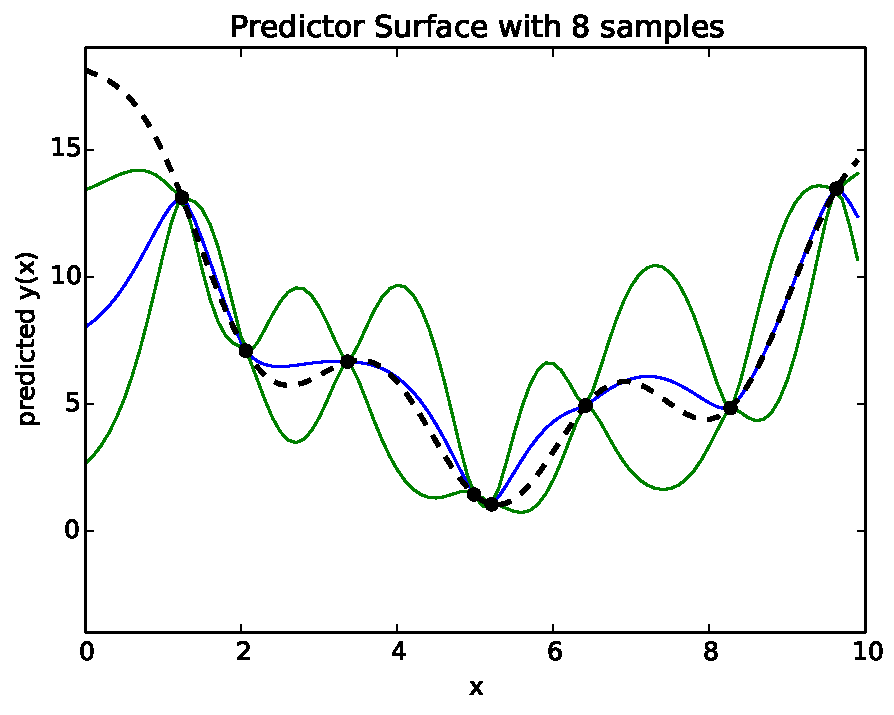
\includegraphics[width=\textwidth]{images/likelihood_opt_ex/bad}
                \caption{L-BFGS-B\cite{}, as implemented by \texttt{scipy.optimize.minimize}. }
        \end{subfigure}%
        ~ %add desired spacing between images, e. g. ~, \quad, \qquad, \hfill etc.
          %(or a blank line to force the subfigure onto a new line)
        \begin{subfigure}[t]{0.5\textwidth}
                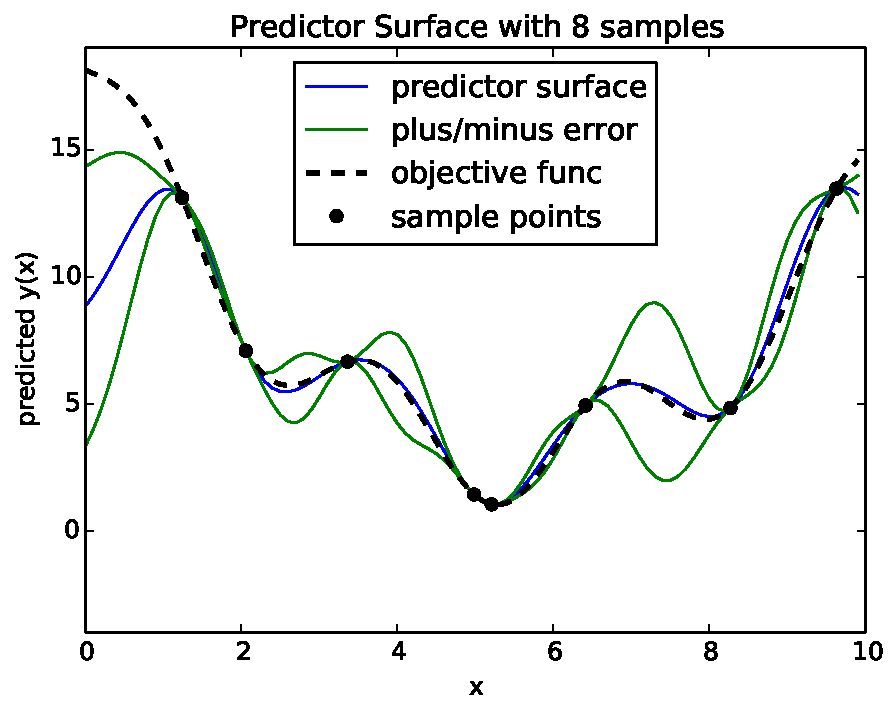
\includegraphics[width=\textwidth]{images/likelihood_opt_ex/good}
                \caption{basinhopping\cite{} global optimization algorithm using COBYLA\cite{} locally, as implemented by \texttt{scipy.optimize.basinhopping}.}
        \end{subfigure}
        \caption{Two DACE predictor models fit to identical sample points, differings only in their method of numeric maximization (labelled) of the parameter likelihood function (Eq. \ref{eq:conc_likelihood}). }\label{fig:opt_compare}
\end{figure}

The optimality of SMBO results depends indirectly, but crucially, on the optimality of the results of these sub-optimizers. The cyclical process works because of each successive model's predictive power in finding the global optimum. The loop is run until, by considering the expected improvement surface, our confidence in having found the global optimum passes a certain threshold. From this we can see that bad predictive models make for an inefficient SMBO loop, because expected improvement is monotonically fixed to predicted error, i.e., more model error means more expected improvement. Poor sub-optimizers make for bad models, which have poor predictive power, which means the SMBO loop will be iterated more times before halting, meaning more calls of the objective function. So, a bad optimizer subroutine will require the objective function to be evaluated more times to get a satisfactory solution to the overall optimization problem. As the premise of this thesis involves a too-expensive blackbox function, this is, of course, bad.

%
%\subsection{Basic Runtime Analysis} \label{sec:runtime}

%Because the premise of this thesis is of an inconveniently-expensive blackbox function, the relevant runtime parameter in this analysis will be the number of objective function evaluations $n$. For convenience, I'll assume that each cycle of the SMBO loop selects only one new sample point, so $n$ is equal to the number of overall SMBO loop iterations.




\chapter{Discussion}

Having presented the general framework of Sequential Model-Based Optimization, and explored the case study of the EGO algorithm, I will here discuss the significance of this optimization paradigm---the types of problems it is equipped to handle, why those problems are here to stay, and why sequential model-based optimization is a conceptually important approach to consider. To do so, I will first survey SMBO algorithms beyond EGO, to give an impression of the state-of-the art. This will lead to a discussion of the \emph{algorithm selection problem}, a particular type of NP-hard search that is of central importance to the field of machine learning. I argue for adopting SMBO as the default solution strategy. Finally, taking a different tack, I will discuss several yet-untested generalizations of SMBO which merit further study, including a strategy I call recursive meta-optimization.

\section{SMBO beyond EGO}

Recall the three-stage characterization of SMBO, most recently illustrated in Section \ref{sec:design}. The first step in this process relies only upon the function being optimized; it is independent of the particulars of the SMBO algorithm at hand. And as discussed at the end of Chapter \ref{ch:smbo} [NOTE: add this important discussion to ch2], the expected improvement function (Eq. \ref{}), whose maximization comrpises the third stage in the process, is a statistical (i.e., mathematical) property which is entirely determined by $\hat{y}$ and $\hat{err}_{\hat{y}}$. This all amounts to say that on the most basic level, the set of SMBO functions varies only in the modelling dimension, the second step of the SMBO process.

In this characterization, an SMBO process is defined by its modelling module. In the EGO function, the DACE model fills this role. Thus, a simple way to think about SMBO in general is as EGO, but with a different model than DACE. The code constructed for this thesis, discussed in Chapter \ref{ch:code} and documented in the code appendix [CITE], is modularized with the primary goal of constructing SMBO processes in this way. That code, like step two above, requires some modeller,

\begin{equation} \label{eq:modeller}
M:\ (\mathbf{X},\mathbf{Y})\rightarrow (\hat{y},\hat{err}_{\hat{y}}),
\end{equation}
which maps sets of sample points (denoted by vector of every tested input $\mathbf{X}$ and the vector of corresponding outputs $\mathbf{Y}$) to predictor and predicted error functions.

First, I'll discuss simple generalizations of EGO/DACE as presented in Jones et al---notably, considering discrete input dimensions.

Then I will survey a few alternative choices of modeller $M$. This discussion will highlight that there are many algorithmic candidates for producing a prediction function given a set of sample points, but in many cases a predicted error function is less accessible. For example, a neural network produces a prediction model from a set of sample points via supervised learning, but it is at first unclear how to quantify the accuracy of that network's prediction on a novel sample.


\section{A Rival to Genetic Algorithms}

(Me jotting down an idea): There is a cool conceptual case to be made that SMBO is a `super GA' (my friends at the PSU lab call it such). Basically, a new sample point in a GA is chosen by random combination and mutation of two previous sample points. SMBO is much more intelligent than random combination/mutation. In the evolution analogy, GAs are like normal two-parental evolution. But if you see SMBO through the evolutionary lens, you could say that each new organism born to the population, rather than being a random child of two parents, is a deliberate, carefully engineered hybrid of all previous organisms who have ever lived. While GAs throw away information with every generation, SMBO reasons about all previous evaluations of the fitness/objective function. SMBOs are also intuitively much better at getting around local optima than GAs, whose only hope of escaping a local optimum is a perfectly-directed random mutation.


\section{The Algorithm Selection Problem}

It is this problem that highlights the relevance of SMBO to machine learning today---given a particular problem or problem type, and a set of algorithms which are candidates for solving that problem, how to you select the best solver? This problem should be of obvious importance to anyone who has practiced machine learning---indeed, it is a large part of the task of solving problems with ML in practice.

I have a good source by Michael Littman (I took an intro to ML MOOC from him!) about solving the ALP with reinforcement learning---I'll steal from him some arguments/citations for why this problem is so important, and emphasize why the ``sample the objective function to maximize expected improvement'' component of SMBO balances exploration/exploitation to make it more desirable than Littman's methods.



\bibliographystyle{apalike}
\bibliography{bib/thesis}


\end{document}



